\chapter{Evaluation}
\label{chapter:evaluation}

% \definecolor{win}{HTML}{0de929}
% \definecolor{loss}{HTML}{ef4748}
\definecolor{win}{HTML}{63be7b}
\definecolor{loss}{HTML}{f8696b}

Nachfolgend wird eine Evaluation der einzelnen Computerengines vorgenommen. Dazu spielen die Computerengines erst einmal verschiedene Vergleichsspiele untereinander. Die Vergleichsspiele sind dabei alle auf einem System mit folgenden Spezifikationen ausgeführt worden:

\begin{itemize}
    \item \vspace{-0.15cm} \textbf{Prozessor:} \ac{AMD} Ryzen 7 5800X 8-Core Processor
    \item \vspace{-0.15cm} \textbf{Arbeitsspeicher:} 32 \acsp{GiB} @ 3600 \acsp{MHz}
    \item \vspace{-0.15cm} \textbf{Betriebssystem:} Windows 11
    \item \vspace{-0.15cm} \textbf{Rust Version:} rustc 1.77.2
\end{itemize}

Sofern nicht anders beschrieben, werden immer 100 Vergleichsspiele zwischen 2 Spielern gegeneinander gespielt. Dabei hat jeder Spieler immer eine Bedenkzeit von $10\acs{s}$, um eine Aktion auszuwählen. Computerengines mit Parallelisierung stehen 8 Threads zur Verfügung.

Die Stichprobe von 100 Spielen ist zu klein, um verlässliche statistische Vorhersagen zu treffen, vor allem, was die genauen Gewinnraten der Spieler gegeneinander betrifft. Eine Tendenz der Ergebnisse lässt sich aber dennoch feststellen. Die kleine Anzahl an Vergleichsspielen ergibt sich aus der zeitlichen und hardwaretechnischen Ressourcenbegrenzung. Ein Spieler hat $10\acs{s}$ Bedenkzeit, multipliziert mit der durchschnittlichen Anzahl an \hyperref[text:ply]{\emph{Plys}} ($42{,}8176$) und den 100 Vergleichsspielen, ergibt sich eine Zeit von ca. $11,89$ Stunden für ein Vergleich zwischen zwei Spielern. Hardwaretechnisch werden alle Spiele auf dem gleichen oben genannten Rechnersystem durchgeführt, um vergleichbare Ergebnisse zu erhalten. Somit war es nicht möglich für die Evaluation mehr Vergleichsspiele durchzuführen. Bei den Vergleichsspielen wird immer nur das Endergebnis (also Gewinnen oder Verlieren) betrachtet, nicht die genaue Endwertung. In tatsächlichen Spielen geht es auch darum welcher Spieler gewinnt und nicht mit welcher Punktzahl. Außerdem wird die genaue Endwertung stark durch die initiale Flickenverteilung, den Spielverlauf und das Gegnerverhalten bestimmt. Spielen zwei starke Spieler gegeneinander, kann die Endwertung niedriger ausfallen als bei zwei schwächeren Spielern, da sich die starken Spieler vielleicht auch gegenseitig die besten Aktionen verbauen.

\begin{figure}[!ht]
    \centering
    \resizebox{\textwidth}{!}{\begin{tikzpicture}
            \coordinate (bar1Start) at (0,0);
            \coordinate (bar1End) at (10,0);
            \coordinate (bar1Break) at (2.1,0);

            \draw[color=win, line width=0.25cm] (bar1Start) -- (bar1Break);
            \draw[color=loss, line width=0.25cm] (bar1Break) -- (bar1End);
            \node[left = 0.1cm of bar1Start] {Random Player};
            \node[right = 0.1cm of bar1End, align=left] {Greedy Player \\ (eval: static)};
            \node[above right = 0.05cm and -0.15cm of bar1Start] {\footnotesize $21$ Gewonnen};
            \node[below = 0.1cm of bar1Break] {\scriptsize $21\%$};
            \node[above left = 0.05cm and -0.15cm of bar1End] {\footnotesize $79$ Verloren};
        \end{tikzpicture}}
    % \vspace*{-0.5cm}
    \caption{Random Player vs. Greedy Player}
    \label{fig:random-greedy-comparison}
\end{figure}

Die Evaluation beginnt mit einem einfachen Vergleich zwischen dem Random Spieler und dem Greedy Spieler mit dem statischen Evaluator. Die Ergebnisse der Vergleichsspiele sind in Abbildung \ref{fig:random-greedy-comparison} dargestellt. Wie zu erwarten, schneidet der Random Spieler schlechter ab als der Greedy Spieler mit 21 Gewonnenen und 79 Verlorenen Spielen. Somit kann in allen nachfolgenden Vergleichen angenommen werden, dass der Random Spieler eine Basis ist, die vermutlich jede andere Engine überwinden kann und der Greedy Player ein guter etwas anspruchsvollerer Vergleichspartner ist.

\section{Vergleich der PVS-Varianten}

Beim \ac{PVS} Spieler werden zuerst während der Suche typische Statistiken betrachtet. Die in Abbildung \ref{fig:pvs-statistics} gezeigten Werte stammen dabei aus einem tatsächlich stattgefundenen Spiel, sind aber vergleichbar mit in anderen Spielen beobachteten Werten.

% ┌───────────────────────────── Principal Variation Search Player ─────────────────────────────┐
% │ Features:            [AW, TT(S), LMR, LMP, SE]                                              │
% │ Depth:               9 started from (P1: 11, P2: 13, type: Normal)                            │
% │ Time:                5.0634892s                                                             │
% │ Nodes searched:      43720                                                                  │
% │ Branching factor:    2.84 AVG / 1.78 EFF / 1.38 MEAN                                        │
% │ Best Action:         P7I1═4‖3↻1↔0P1 (3 points)                                              │
% │ Move Ordering:       86.80\% (8611 high pv / 9920 high)                                      │
% │ Aspiration window:   0 low / 0 high                                                         │
% │ Zero window search:  2 fails (0.01\%)                                                        │
% │ Search Extensions:   1 SP, 0 ST (enabled)                                                   │
% │ LMR (Fail/All):      0/114 (0.00%)                                                          │
% │ LMP:                 3271                                                                   │
% │ Principal Variation: P7I1═4‖3↻1↔0P1 → P21I0═2‖1↻0↔0P0 → P31I0═7‖4↻0↔1P1 → P11I0═0‖2↻0↔1P0 │
% │ ┌──────────────────────────── Transposition Table Statistics ─────────────────────────────┐ │
% │ │ Capacity:            10416666                                                           │ │
% │ │ Entries:              5257801 /  50.47\% filled                                          │ │
% │ │ Overwrites:          13138704                                                           │ │
% │ │ Accesses:             1141676                                                           │ │
% │ │ ├──► Hit:              261862 /  22.94\%                                                 │ │
% │ │ └──► Miss:             879814 /  77.06\%                                                 │ │
% │ └─────────────────────────────────────────────────────────────────────────────────────────┘ │
% └─────────────────────────────────────────────────────────────────────────────────────────────┘
\begin{figure}[!ht]
    \centering
    \resizebox{\textwidth}{!}{\begin{tcolorbox}[
                rounded corners=all,
                boxrule=1pt,
                colback=white,
                colframe=black,
                hbox,
                % width=\linewidth,
                enhanced,
                coltitle=black,
                title={\acl{PVS} Player},
                top=6pt,
                left=0pt,
                right=5pt,
                bottom=0pt,
                attach boxed title to top center={yshift=-\tcboxedtitleheight/2},
                boxed title style={size=small,colback=white,colframe=white}
            ]
            \begingroup
            \setlength{\arrayrulewidth}{0pt}

            \begin{tabular}{@{}ll@{}}
                Features:             & [AW, TT(S), \acs{LMR}, \acs{LMP}, SE]                                \\
                Depth:                & $9$ started from (P1: $11$, P2: $13$, type: Normal)                  \\
                Time:                 & $5{,}0634892\acs{s}$                                                 \\
                Nodes searched:       & $43720$                                                              \\
                % Branching factor:   & $2{,}84$ AVG / $1{,}78$ EFF / $1{,}38$ MEAN                          \\
                % Branching factor:     & $13{,}73$ AVG / $3{,}32$ EFF / $1{,}59$ MEAN                         \\
                Best Action:          & P7I1═4‖3↻1↔0P1 ($3$ points)                                          \\
                Action Ordering:      & $86{,}80\%$ ($8611$ high pv / $9920$ high)                           \\
                Aspiration window:    & $0$ low / $0$ high                                                   \\
                Zero window search:   & $2$ fails ($0{,}01\%$)                                               \\
                Search Extensions:    & $1$ SP, $0$ ST (enabled)                                             \\
                \acs{LMR} (Fail/All): & $0/114$ ($0{,}00\%$)                                                 \\
                \acs{LMP}:            & $3271$                                                               \\
                \acl{PV}:             & P7I1═4‖3↻1↔0P1 → P21I0═2‖1↻0↔0P0 → P31I0═7‖4↻0↔1P1 → P11I0═0‖2↻0↔1P0 \\
                \multicolumn{2}{@{}c@{}}{
                \begin{tcolorbox}[
                        rounded corners=all,
                        boxrule=1pt,
                        colback=white,
                        colframe=black,
                        width=1.325\linewidth,
                        enhanced,
                        coltitle=black,
                        title={Transposition Table},
                        top=6pt,
                        left=0pt,
                        right=0pt,
                        bottom=0pt,
                        attach boxed title to top center={yshift=-\tcboxedtitleheight/2},
                        boxed title style={size=small,colback=white,colframe=white}
                    ]
                    \begin{tabular}{ll}
                        Capacity:   & $10416666$                      \\
                        Entries:    & $5257801$ /  $50{,}47\%$ filled \\
                        Overwrites: & $13138704$                      \\
                        Accesses:   & $1141676$                       \\
                        ├──► Hit:   & $261862$ /  $22{,}94\%$         \\
                        └──► Miss:  & $879814$ /  $77{,}06\%$         \\
                    \end{tabular}
                \end{tcolorbox}
                }                                                                                            \\
            \end{tabular}
            \endgroup
        \end{tcolorbox}}
    \vspace*{-0.25cm}
    \caption[PVS-Suchstatistiken]{\acs{PVS}-Suchstatistiken}
    \label{fig:pvs-statistics}
\end{figure}

Der \ac{PVS} Spieler schafft in der Regel eine Suchtiefe von 8 bis 11 Ebenen. Dabei werden nach 10 Sekunden ca. $150{.}000$ Knoten bzw. Spielzustände durchsucht und evaluiert. Neben der besten Aktion, welche durch den \ac{PVS} Spieler ausgewählt wird, kann auch die gesamte \acs{PV} betrachtet werden, welche sich über mehrere Ebenen erstreckt. Die Aktionen Anordnung ist im $80\%-90\%$ akzeptabel, aber noch verbesserbar. Generell findet ein \hyperref[text:beta-cutoff]{\emph{Beta-Cutoff}} fast immer am ersten Knoten statt, was für eine gelungene Umsetzung von \ac{PVS} spricht. Die Aspiration Window Funktionalität verkleinert das Suchfenster und muss nur in wenigen Fällen erneut Suchen (in \ref{fig:pvs-statistics} kein einziges Mal). Auch die Sucherweiterungen, \ac{LMR} und \ac{LMP} funktionieren, wobei vor allem durch \ac{LMP} sehr viele Teilbäume gar nicht evaluiert werden (in der Statistik 3271). Die Transpositionstabelle hat eine \emph{Hit-Rate} von $\approx 23\%$, was nicht sehr viel ist. Dies ist für Patchwork aber auch zu erwarten, da es zum Beispiel im Gegensatz zu Schach, kaum Zugfolgen gibt, die im gleichen Spielzustand enden. Dies ist der Fall, da man entweder direkt 2 Flicken nacheinander auswählen kann oder zuerst den zweiten Flicken nimmt und dann eine ganze Umrundung der Flicken mit der Spielfigur abwarten muss, um den gleichen zweiten Flicken zu nehmen. Die Wahrscheinlichkeit, dass in diesem Fall auch der Knopfvorrat, Position auf dem Zeitplan und alle weiteren Eigenschaften gleich sind, ist gering. Das Einfügen von Position mit Symmetrie erhöht die \emph{Hit-Rate} nur um etwa $2\%$, eine kleine, aber dennoch bedeutungsvolle Änderung.

In Abbildung \ref{fig:pvs-comparision} werden die einzelnen Funktionalitäten des \ac{PVS} Spielers getestet, indem immer ein Spieler mit allen aktivierten Funktionalitäten gegen einen anderen Spieler antritt, bei dem eine der Funktionalitäten abgeschaltet ist.

\begin{figure}[!ht]
    \centering
    \resizebox{\textwidth}{!}{\begin{tikzpicture}
            % \coordinate (bar1Start) at (0,0);
            % \coordinate (bar1End) at (10,0);
            % \coordinate (bar1Break) at (6.4,0);

            % \draw[color=win, line width=0.25cm] (bar1Start) -- (bar1Break);
            % \draw[color=loss, line width=0.25cm] (bar1Break) -- (bar1End);
            % \node[left = 0.1cm of bar1Start] {Hard-Fail};
            % \node[right = 0.1cm of bar1End] {Soft-Fail};
            % \node[above right = 0.05cm and -0.15cm of bar1Start] {\footnotesize $64$ Gewonnen};
            % \node[below = 0.1cm of bar1Break] {\scriptsize $64\%$};
            % \node[above left = 0.05cm and -0.15cm of bar1End] {\footnotesize $36$ Verloren};

            \coordinate (bar2Start) at (0,0);
            \coordinate (bar2End) at (10,0);
            \coordinate (bar2Break) at (5.1,0);

            \draw[color=win, line width=0.25cm] (bar2Start) -- (bar2Break);
            \draw[color=loss, line width=0.25cm] (bar2Break) -- (bar2End);
            \node[left = 0.1cm of bar2Start] {AspirationWindow};
            \node[right = 0.1cm of bar2End] {Kein AspirationWindow};
            \node[above right = 0.05cm and -0.15cm of bar2Start] {\footnotesize $51$ Gewonnen};
            \node[below = 0.1cm of bar2Break] {\scriptsize $51\%$};
            \node[above left = 0.05cm and -0.15cm of bar2End] {\footnotesize $49$ Verloren};

            \coordinate (bar3Start) at (0,-1.5);
            \coordinate (bar3End) at (10,-1.5);
            \coordinate (bar3Break) at (5.4,-1.5);

            \draw[color=win, line width=0.25cm] (bar3Start) -- (bar3Break);
            \draw[color=loss, line width=0.25cm] (bar3Break) -- (bar3End);
            \node[left = 0.1cm of bar3Start] {Sucherweiterungen};
            \node[right = 0.1cm of bar3End] {Keine Sucherweiterungen};
            \node[above right = 0.05cm and -0.15cm of bar3Start] {\footnotesize $54$ Gewonnen};
            \node[below = 0.1cm of bar3Break] {\scriptsize $54\%$};
            \node[above left = 0.05cm and -0.15cm of bar3End] {\footnotesize $46$ Verloren};

            \coordinate (bar4Start) at (0,-3);
            \coordinate (bar4End) at (10,-3);
            \coordinate (bar4Break) at (5.3,-3);

            \draw[color=win, line width=0.25cm] (bar4Start) -- (bar4Break);
            \draw[color=loss, line width=0.25cm] (bar4Break) -- (bar4End);
            \node[left = 0.1cm of bar4Start] {\acs{LMR}, \acs{LMP}};
            \node[right = 0.1cm of bar4End] {Kein \acs{LMR}, \acs{LMP}};
            \node[above right = 0.05cm and -0.15cm of bar4Start] {\footnotesize $53$ Gewonnen};
            \node[below = 0.1cm of bar4Break] {\scriptsize $53\%$};
            \node[above left = 0.05cm and -0.15cm of bar4End] {\footnotesize $47$ Verloren};

            \coordinate (bar5Start) at (0,-4.5);
            \coordinate (bar5End) at (10,-4.5);
            \coordinate (bar5Break) at (5,-4.5);

            \draw[color=win, line width=0.25cm] (bar5Start) -- (bar5Break);
            \draw[color=loss, line width=0.25cm] (bar5Break) -- (bar5End);
            \node[left = 0.1cm of bar5Start] {Table Ordering};
            \node[right = 0.1cm of bar5End] {Static Eval Ordering};
            \node[above right = 0.05cm and -0.15cm of bar5Start] {\footnotesize $50$ Gewonnen};
            \node[below = 0.1cm of bar5Break] {\scriptsize $50\%$};
            \node[above left = 0.05cm and -0.15cm of bar5End] {\footnotesize $50$ Verloren};

            \coordinate (bar6Start) at (0,-6);
            \coordinate (bar6End) at (10,-6);
            \coordinate (bar6Break) at (4.1,-6);

            \draw[color=win, line width=0.25cm] (bar6Start) -- (bar6Break);
            \draw[color=loss, line width=0.25cm] (bar6Break) -- (bar6End);
            \node[left = 0.1cm of bar6Start] {Kein \acs{SMP}};
            \node[right = 0.1cm of bar6End] {Lazy \acs{SMP}};
            \node[above right = 0.05cm and -0.15cm of bar6Start] {\footnotesize $41$ Gewonnen};
            \node[below = 0.1cm of bar6Break] {\scriptsize $41\%$};
            \node[above left = 0.05cm and -0.15cm of bar6End] {\footnotesize $59$ Verloren};
        \end{tikzpicture}}
    % \vspace*{-0.5cm}
    \caption[Vergleich der PVS Varianten]{Vergleich der \acs{PVS} Varianten}
    \label{fig:pvs-comparision}
\end{figure}

Mit Aspiration Windows aktiviert gewinnt der \ac{PVS} Spieler $51\%$ der Spiele gegen sich selbst. Bei 100 Spielen ist dies keine Garantie für eine Verbesserung, legt aber zumindest nahe, dass sich die Performance nicht verschlechtert hat. Die Sucherweiterungen sowie \ac{LMR} und \ac{LMP} bringen einen kleinen aber gleichzeitig bemerkbaren Vorteil. Weiterhin wurde die Aktionen Anordnung getestet. Ein Spieler spielt mit der normalen auf Tabellenwerten basierten Aktionen-Anordnung, während ein anderer Spieler die tatsächliche Evaluation des statischen Evaluierers verwendet, um die Aktionen anzuordnen (außer für die \ac{PV} Aktion, welche immer an die erste Stelle angeordnet wird). Das Ergebnis beträgt dabei $50\%$, was dafürspricht, dass die Standard-Tabellenanordnung die Aktionen bereits relativ gut anordnet. Auf jeden Fall kann der statische Evaluierer die Aktionen auch nicht besser anordnen. Zuletzt gibt es noch einen Vergleich zwischen dem Single-Threaded-\ac{PVS}-Spieler und der Variante mit Lazy \ac{SMP}. Diesen Vergleich gewinnt die parallelisierte Lazy \ac{SMP} Variante.

\section{Vergleich der MCTS-Varianten}

Im diesem Abschnitt werden die einzelnen Varianten des \ac{MCTS} Spielers miteinander verglichen. Zuerst sind dabei alle Tree Policies sowie Evaluatoren in der Tabelle \ref{tabelle:mcts-policy-eval-comparision} aufgelistet. Dabei tritt jede Kombination gegen jede andere Kombination an. In den einzelnen Zellen ist das Ergebnis der Vergleichsspiele als Gewinnrate zwischen 0 und 1 aus Sicht des Zeilenspielers aufgetragen (So gewinnt beispielsweise \emph{\acs{UCT},Win} mit $56{,}2\%$ gegen \emph{\acs{UCT},Score}). Die Vergleichsspiele umfassen dabei immer 1000 Spiele mit je 2500 Iterationen pro \hyperref[text:ply]{\emph{Ply}}. Um möglichst vergleichbare Spiele sicherzustellen, werden keine Suchbäume wiederverwendet und es findet auch keine Parallelisierung der einzelnen \ac{MCTS} Varianten statt.

\begin{table}[H]
    \centering
    \resizebox{\textwidth}{!}{\begin{tabular}{|c|c|c|c|c|c|c|c|c|c|c|}
            \hline
            \multicolumn{1}{|c}{Policy}       & $\rightarrow$ & \ac{UCT}                          & \ac{UCT}                          & \ac{UCT}                          & Score                             & Score                             & Score                             & \tiny \makecell{Partial-                                                                                  \\Score}  & \tiny \makecell{Partial-\\Score}  & \tiny \makecell{Partial-\\Score}  \\ \cline{3-11}
            \multicolumn{1}{|c}{$\downarrow$} & Evaluator     & Win                               & Score                             & Static                            & Win                               & Score                             & Static                            & Win                               & Score                             & Static                            \\ \hline
            \ac{UCT}                          & Win           & $\diagup$                         & \cellcolor[HTML]{ece683}$0{,}562$ & \cellcolor[HTML]{67bf7c}$0{,}989$ & \cellcolor[HTML]{c5db81}$0{,}686$ & \cellcolor[HTML]{fee883}$0{,}490$ & \cellcolor[HTML]{85c87d}$0{,}894$ & \cellcolor[HTML]{f3e884}$0{,}541$ & \cellcolor[HTML]{f7e984}$0{,}526$ & \cellcolor[HTML]{82c77d}$0{,}902$ \\ \hline
            \ac{UCT}                          & Score         & \cellcolor[HTML]{feda80}$0{,}438$ & $\diagup$                         & \cellcolor[HTML]{68c07c}$0{,}984$ & \cellcolor[HTML]{cadc81}$0{,}673$ & \cellcolor[HTML]{fbea84}$0{,}516$ & \cellcolor[HTML]{7ec67d}$0{,}914$ & \cellcolor[HTML]{f7e984}$0{,}526$ & \cellcolor[HTML]{feea83}$0{,}499$ & \cellcolor[HTML]{85c87d}$0{,}894$ \\ \hline
            \ac{UCT}                          & Static        & \cellcolor[HTML]{f86b6b}$0{,}011$ & \cellcolor[HTML]{f86d6b}$0{,}016$ & $\diagup$                         & \cellcolor[HTML]{f8726c}$0{,}038$ & \cellcolor[HTML]{f86d6b}$0{,}018$ & \cellcolor[HTML]{fcb87a}$0{,}305$ & \cellcolor[HTML]{f86e6c}$0{,}021$ & \cellcolor[HTML]{f86c6b}$0{,}013$ & \cellcolor[HTML]{fcb87a}$0{,}304$ \\ \hline
            Score                             & Win           & \cellcolor[HTML]{fcba7a}$0{,}314$ & \cellcolor[HTML]{fcbe7b}$0{,}327$ & \cellcolor[HTML]{6fc27c}$0{,}962$ & $\diagup$                         & \cellcolor[HTML]{fdca7d}$0{,}374$ & \cellcolor[HTML]{a0d07f}$0{,}805$ & \cellcolor[HTML]{fcc07b}$0{,}335$ & \cellcolor[HTML]{fcc47c}$0{,}353$ & \cellcolor[HTML]{9dcf7f}$0{,}816$ \\ \hline
            Score                             & Score         & \cellcolor[HTML]{fceb84}$0{,}510$ & \cellcolor[HTML]{fee683}$0{,}484$ & \cellcolor[HTML]{69c07c}$0{,}982$ & \cellcolor[HTML]{d8e082}$0{,}626$ & $\diagup$                         & \cellcolor[HTML]{7ec67d}$0{,}915$ & \cellcolor[HTML]{f6e984}$0{,}531$ & \cellcolor[HTML]{fbea84}$0{,}516$ & \cellcolor[HTML]{80c77d}$0{,}909$ \\ \hline
            Score                             & Static        & \cellcolor[HTML]{f98470}$0{,}106$ & \cellcolor[HTML]{f97f6f}$0{,}086$ & \cellcolor[HTML]{c3da81}$0{,}695$ & \cellcolor[HTML]{fa9b74}$0{,}195$ & \cellcolor[HTML]{f97f6f}$0{,}085$ & $\diagup$                         & \cellcolor[HTML]{f98871}$0{,}123$ & \cellcolor[HTML]{f9806f}$0{,}092$ & \cellcolor[HTML]{fedf81}$0{,}457$ \\ \hline
            \tiny \makecell{Partial-                                                                                                                                                                                                                                                                                                                                                              \\Score} &           Win & \cellcolor[HTML]{fee081}$0{,}459$ & \cellcolor[HTML]{fee482}$0{,}474$ & \cellcolor[HTML]{6ac07c}$0{,}979$ & \cellcolor[HTML]{ccdd82}$0{,}665$ & \cellcolor[HTML]{fee282}$0{,}469$ & \cellcolor[HTML]{8aca7e}$0{,}877$ & $\diagup$                         & \cellcolor[HTML]{fbea84}$0{,}513$ & \cellcolor[HTML]{82c77d}$0{,}903$ \\ \hline
            \tiny \makecell{Partial-                                                                                                                                                                                                                                                                                                                                                              \\Score} &         Score & \cellcolor[HTML]{fee482}$0{,}474$ & \cellcolor[HTML]{ffeb84}$0{,}501$ & \cellcolor[HTML]{68c07c}$0{,}987$ & \cellcolor[HTML]{d2de82}$0{,}647$ & \cellcolor[HTML]{fee683}$0{,}484$ & \cellcolor[HTML]{80c77d}$0{,}908$ & \cellcolor[HTML]{fee783}$0{,}487$ & $\diagup$                         & \cellcolor[HTML]{7cc67d}$0{,}920$ \\ \hline
            \tiny \makecell{Partial-                                                                                                                                                                                                                                                                                                                                                              \\Score} &        Static & \cellcolor[HTML]{f9826f}$0{,}098$ & \cellcolor[HTML]{f98470}$0{,}106$ & \cellcolor[HTML]{c2da81}$0{,}696$ & \cellcolor[HTML]{fa9874}$0{,}184$ & \cellcolor[HTML]{f9806f}$0{,}091$ & \cellcolor[HTML]{f2e884}$0{,}543$ & \cellcolor[HTML]{f9826f}$0{,}097$ & \cellcolor[HTML]{f97d6e}$0{,}080$ & $\diagup$                         \\ \hline
        \end{tabular}}
    \vspace{3pt}
    \caption{Vergleich der \acs{MCTS} Policy und Evaluator Varianten}
    \label{tabelle:mcts-policy-eval-comparision}
\end{table}

Wie in Tabelle \ref{tabelle:mcts-policy-eval-comparision} zu sehen ist, sind viele der Varianten sehr vergleichbar. So gewinnt die \emph{\acs{UCT},Win} Variante beispielsweise gegen alle anderen Varianten außer \emph{Score,Score}. Die \emph{Score,Score} Variante hingegen verliert gegen die \emph{\acs{UCT},Score} Variante, die wiederrum gegen die \emph{\acs{UCT},Win} Variante verliert. Die einzigen Varianten, welche eine deutlich schlechtere Leistung erbringen ist \emph{Score,Win} und alle Varianten mit dem statischen Evaluator. Die \emph{Score,Win} Variante erzeugt innerhalb der Simulationsphase immer das Ergebnis $-1$ oder $1$. Auf Basis dieser zwei Werte erzeugt die Score-Tree-Policy eine Auswahl der Knoten innerhalb der Selektionsphase, was natürlich nicht sehr aussagekräftig ist, womit auch das schlechtere Abschneiden erklärt ist. Die statische Evaluation wurde nur eingesetzt, weil es möglich ist. Jedoch widerspricht diese statische Evaluation gerade dem Prinzip, wodurch der \ac{MCTS} Spieler seine Stärke erreicht: Möglichst viele Iterationen durchführen, um somit den wahren Wert einer Aktion durch eine genügend große Stichprobe an Spielverläufen ausreichend gut zu approximieren. Der statische Evaluator bricht den Vorgang verführt ab, um die Stichproben durch eine immer gleichbleibende und verzerrte Evaluation zu ersetzen. Somit ähnelt diese Variante eher dem \ac{PVS} Spieler der nur ein paar Ebenen tief schauen kann und schneidet deutlich schlechter ab als die tatsächlichen \ac{MCTS} Varianten. Die tatsächlichen Varianten sind aber recht ähnlich. Aus diesem Grund wurde die \emph{Partial-Score} Tree Policy auch nur einmal mit $\rho = 10\%$ in die Tabelle mit aufgenommen. Nachfolgend wird deshalb auch einfach zufällig die \emph{\acs{UCT},Win} Variante für die Vergleiche weiterverwendet .

\begin{figure}[!ht]
    \centering
    \begin{tikzpicture}
        \node at (5,0) [align=center] {$5{.}000$ Iterationen mit $2\acs{ms}$ Tree Reuse Timeout};

        \coordinate (bar1Start) at (0,-1);
        \coordinate (bar1End) at (10,-1);
        \coordinate (bar1Break) at (5,-1);

        \draw[color=win, line width=0.25cm] (bar1Start) -- (bar1Break);
        \draw[color=loss, line width=0.25cm] (bar1Break) -- (bar1End);
        \node[left = 0.1cm of bar1Start] {Tree New};
        \node[right = 0.1cm of bar1End] {Tree Reuse};
        \node[above right = 0.05cm and -0.15cm of bar1Start] {\footnotesize $500$ Gewonnen};
        \node[below = 0.1cm of bar1Break] {\scriptsize $50\%$};
        \node[above left = 0.05cm and -0.15cm of bar1End] {\footnotesize $500$ Verloren};

        \node at (5,-2.25) [align=center] {$100{.}000$ Iterationen};

        \coordinate (bar2Start) at (0,-3);
        \coordinate (bar2End) at (10,-3);
        \coordinate (bar2Break) at (4.99,-3);

        \draw[color=win, line width=0.25cm] (bar2Start) -- (bar2Break);
        \draw[color=loss, line width=0.25cm] (bar2Break) -- (bar2End);
        \node[left = 0.1cm of bar2Start] {Tree New};
        \node[right = 0.1cm of bar2End] {Tree Reuse};
        \node[above right = 0.05cm and -0.15cm of bar2Start] {\footnotesize $499$ Gewonnen};
        \node[below = 0.1cm of bar2Break] {\scriptsize $49{,}9\%$};
        \node[above left = 0.05cm and -0.15cm of bar2End] {\footnotesize $501$ Verloren};
    \end{tikzpicture}
    % \vspace*{-0.5cm}
    \caption[Vergleich Baumwiederverwendung bei MCTS]{Vergleich neuer Baum vs. Baum wiederverwenden bei \acs{MCTS}}
    \label{fig:mcts-tree-reuse-comparision}
\end{figure}

Weiterhin werden die \ac{MCTS} Spielervarianten noch verglichen, indem ein Spieler immer wieder versucht den alten Suchbaum wiederzuverwenden (\emph{Tree Reuse}), während der andere Spieler einfach direkt mit einem neuen Suchbaum anfängt (\emph{Tree New}). Die in \ref{fig:mcts-tree-reuse-comparision} gezeigten Ergebnisse sind dabei relative ernüchternd. Einerseits werden beide Varianten mit $5{.}000$ Iterationen getestet, wobei für \emph{Tree Reuse} ein Timeout von $2\acsp{ms}$ hat, um den neuen Spielzustand im alten Suchbaum zu finden. Andererseits werden beide Varianten noch mit je $100{.}000$ Iterationen pro \hyperref[text:ply]{\emph{Ply}} und keinem Timeout für \emph{Tree Reuse} verglichen. Beide Vergleiche enden dabei mit einer Gewinnrate von ziemlich genau $50\%$. Selbst bei Variante mit vielen Iterationen, bei der immer der Suchbaum wiederverwendet wird, gewinnt \emph{Tree Reuse} nur ein Spiel mehr, was statistisch wenig aussagekräftig ist. Dies ist der Fall, obwohl mehr Iterationen einen größeren Suchbaum und somit auch einen größeren wiederverwendeten Teilbaum implizieren. Wenn das Wiederverwenden des Suchbaums also einen Vorteil bringen sollte, dann ist der Versuchsaufbau oder die Stichprobengröße nicht groß genug, um diesen Vorteil eindeutig abzugrenzen.

\begin{figure}[!ht]
    \centering
    \begin{tikzpicture}
        \coordinate (bar1Start) at (0,0);
        \coordinate (bar1End) at (10,0);
        \coordinate (bar1Break) at (7.7,0);

        \draw[color=win, line width=0.25cm] (bar1Start) -- (bar1Break);
        \draw[color=loss, line width=0.25cm] (bar1Break) -- (bar1End);
        \node[left = 0.1cm of bar1Start, align=right] {\acs{MCTS}\\(1 Thread)};
        \node[right = 0.1cm of bar1End, align=left] {\acs{MCTS}\\(8 Leaf)};
        \node[above right = 0.05cm and -0.15cm of bar1Start] {\footnotesize $77$ Gewonnen};
        \node[below = 0.1cm of bar1Break] {\scriptsize $77\%$};
        \node[above left = 0.05cm and -0.15cm of bar1End] {\footnotesize $23$ Verloren};

        \coordinate (bar2Start) at (0,-1.5);
        \coordinate (bar2End) at (10,-1.5);
        \coordinate (bar2Break) at (4.6,-1.5);

        \draw[color=win, line width=0.25cm] (bar2Start) -- (bar2Break);
        \draw[color=loss, line width=0.25cm] (bar2Break) -- (bar2End);
        \node[left = 0.1cm of bar2Start, align=right] {\acs{MCTS}\\(1 Thread)};
        \node[right = 0.1cm of bar2End, align=left] {\acs{MCTS}\\(8 Root)};
        \node[above right = 0.05cm and -0.15cm of bar2Start] {\footnotesize $46$ Gewonnen};
        \node[below = 0.1cm of bar2Break] {\scriptsize $46\%$};
        \node[above left = 0.05cm and -0.15cm of bar2End] {\footnotesize $54$ Verloren};

        \coordinate (bar3Start) at (0,-3);
        \coordinate (bar3End) at (10,-3);
        \coordinate (bar3Break) at (1.8,-3);

        \draw[color=win, line width=0.25cm] (bar3Start) -- (bar3Break);
        \draw[color=loss, line width=0.25cm] (bar3Break) -- (bar3End);
        \node[left = 0.1cm of bar3Start, align=right] {\acs{MCTS}\\(8 Leaf)};
        \node[right = 0.1cm of bar3End, align=left] {\acs{MCTS}\\(8 Root)};
        \node[above right = 0.05cm and -0.15cm of bar3Start] {\footnotesize $18$ Gewonnen};
        \node[below = 0.1cm of bar3Break] {\scriptsize $18\%$};
        \node[above left = 0.05cm and -0.15cm of bar3End] {\footnotesize $82$ Verloren};
    \end{tikzpicture}
    % \vspace*{-0.5cm}
    \caption[Vergleich der MCTS Varianten]{Vergleich der \acs{MCTS} Varianten}
    \label{fig:mcts-comparision}
\end{figure}

\pagebreak

Um die \ac{MCTS} Spielervergleiche abzuschließen, werden zuletzt die einzelnen Parallelisierungsmöglichkeiten untereinander in \ref{fig:mcts-comparision} verglichen. Dabei spielen die nicht parallelisierte Single-Threaded Variante sowie die Leaf- und Root-Parallelisierten Varianten mit 8 Threads gegeneinander. Die \hyperref[text:leaf-parallelization]{\emph{Leaf Parallelisierung}} schneidet dabei am schlechtesten ab, auch schlechter als die \ac{MCTS} Suche mit einem Thread. Da der \ac{MCTS} Spieler in Patchwork generell sehr wenige Iterationen schafft, ist es wahrscheinlich besser die Change einen guten Spielverlauf zu finden durch viele Iterationen zu maximieren, anstatt weniger Pfade auszuprobieren und für diese Pfade mittels \hyperref[text:leaf-parallelization]{\emph{Leaf Parallelisierung}} eine etwas genaueren Schätzer für den tatsächlichen Wert eines Knotens zu erhalten. Am besten spielt die \hyperref[text:root-parallelization]{\emph{Root-Parallelisierte}} Variante. Diese setzt sich gegen beide anderen Varianten durch, auch wenn der Vorsprung vor der Single-Threaded Variante geringer ausfällt als erhofft.

% ┌───────────────────────────── MCTS Player ─────────────────────────────┐
% │ Features:            [RP(8), RT]                                      │
% │ Duration:            9.925s                                           │
% │ Total Iterations:    592082                                           │
% │ Iterations:          74767                                            │
% │ Nodes:               74791                                            │
% │ Reused Tree:         true                                             │
% │ Root actions:        110                                              │
% │ Expanded Depth:      4                                                │
% │ Win Percentage:      98.40%                                           │
% │ Principal Variation: P17I2═5‖0↻0↔0P1 → W27 → P28I0═8‖1↻0↔0P1 → S═4‖4 │
% │ Min/Max Evaluation:  -1/1                                             │
% └───────────────────────────────────────────────────────────────────────┘
\begin{figure}[!ht]
    \centering
    \resizebox{\textwidth}{!}{\begin{tcolorbox}[
                rounded corners=all,
                boxrule=1pt,
                colback=white,
                colframe=black,
                hbox,
                % width=\linewidth,
                enhanced,
                coltitle=black,
                title={\acs{MCTS} Player},
                top=6pt,
                left=0pt,
                right=3pt,
                bottom=0pt,
                attach boxed title to top center={yshift=-\tcboxedtitleheight/2},
                boxed title style={size=small,colback=white,colframe=white}
            ]
            \begingroup
            \setlength{\arrayrulewidth}{0pt}

            \begin{tabular}{@{}ll@{}}
                Features:           & [RP(8), RT]                                     \\
                Duration:           & $9{,}925\acs{s}$                                \\
                Total Iterations:   & $592082$                                        \\
                Iterations:         & $74767$                                         \\
                Nodes:              & $74791$                                         \\
                Reused Tree:        & true                                            \\
                Root actions:       & $110$                                           \\
                Expanded Depth:     & $4$                                             \\
                Win Percentage:     & $98{,}40\%$                                     \\
                \acl{PV}:           & P17I2═5‖0↻0↔0P1 → W27 → P28I0═8‖1↻0↔0P1 → S═4‖4 \\
                Min/Max Evaluation: & $-1\ /\ 1$                                      \\
            \end{tabular}

            \endgroup
        \end{tcolorbox}}
    \vspace*{-0.25cm}
    \caption[MCTS-Suchstatistiken]{\acs{MCTS}-Suchstatistiken}
    \label{fig:mcts-statistics}
\end{figure}

Abschließend werden wie beim \ac{PVS} Spieler noch verschiedene Statistiken zu einer \ac{MCTS} Suche betrachtet. Die in Abbildung \ref{fig:mcts-statistics} gezeigte Auflistung stammt dabei von einem \ac{MCTS} Spieler mit einer \hyperref[text:root-parallelization]{\emph{Root Parallelisierung}} mit 8 Threads, der seinen Suchbaum wiederverwendet, die \ac{UCT} Tree Policy sowie den Win-Loss-Evaluator verwendet. Generell schafft ein Thread innerhalb der Suchzeit meistens zwischen $50{.}000$ und $100{.}000$ Iterationen. Je später im Spiel eine Aktion gesucht wird, desto mehr Iterationen sind es normalerweise, da eine Simulationsphase zum Beispiel statt $42$ nur noch $10$ \hyperref[text:ply]{\emph{Plys}} umfasst. Über eine Vielzahl von Iterationen summiert sich dieser kleine Zeitunterschied auf. In der dargestellten Auflistung hat der Main-Thread $74{.}767$ Iterationen geschafft.

Es ist auch zu erkennen, dass die \hyperref[text:root-parallelization]{\emph{Root Parallelisierung}} einwandfrei funktioniert. Schafft ein Thread $74{.}767$ Iterationen, so müssten 8 Threads $74{.}767 \cdot 8 = 598{.}136$ Iterationen schaffen. Der tatsächliche Wert aller Threads liegt bei $592{.}082$ Iterationen, was einer prozentualen Abweichung von $-1{,}01\%$ vom erwarteten Wert entspricht und somit innerhalb der Fehlermarge liegt. Auch gibt es im Suchbaum des Main-Threads leicht weniger Knoten als Iterationen im Baum. Somit wurde die Expansionsphase innerhalb einiger Iterationen übersprungen, was nur vorkommen kann, falls ein Spielverlauf verfolgt wird, der im Baum in einem bereits bestehendem Terminalknoten endet. Das ist generell ein gutes Zeichen, da der \ac{MCTS} Spieler in diesem Fall bereit einen großen Bereich der möglichen Spielverläufe erkundet oder einen sehr vielversprechenden Spielverlauf gefunden hat. Die \acl{PV} ist 4 \hyperref[text:ply]{\emph{Plys}} lang. Somit wurden entlang der \ac{PV} vier Ebenen lang alle möglichen Aktionen expandiert und mindestens einmal erkunden. Nach diesen vier Ebenen existieren noch weitere Ebenen, bei denen aber noch nicht alle möglichen Aktionen erkunden sind.

\section{Evaluation von PatchZero}

Die Evaluation des PatchZero Spielers findet im direkten Vergleich mit dem RandomPlayer und dem GreedyPlayer statt (Abbildung \ref{fig:patchzero-comparision}). PatchZero gewinnt gegen RandomPlayer mit einem sehr knappen Vorsprung. Mit so einem kleinen Vorsprung wird PatchZero wie zu erwarten danach eindeutig vom GreedyPlayer geschlagen.

\begin{figure}[!ht]
    \centering
    \begin{tikzpicture}
        \coordinate (bar1Start) at (0,0);
        \coordinate (bar1End) at (10,0);
        \coordinate (bar1Break) at (5.5,0);

        \draw[color=win, line width=0.25cm] (bar1Start) -- (bar1Break);
        \draw[color=loss, line width=0.25cm] (bar1Break) -- (bar1End);
        \node[left = 0.1cm of bar1Start] {PatchZero};
        \node[right = 0.1cm of bar1End] {RandomPlayer};
        \node[above right = 0.05cm and -0.15cm of bar1Start] {\footnotesize $55$ Gewonnen};
        \node[below = 0.1cm of bar1Break] {\scriptsize $55\%$};
        \node[above left = 0.05cm and -0.15cm of bar1End] {\footnotesize $45$ Verloren};

        \coordinate (bar2Start) at (0,-1.5);
        \coordinate (bar2End) at (10,-1.5);
        \coordinate (bar2Break) at (2.2,-1.5);

        \draw[color=win, line width=0.25cm] (bar2Start) -- (bar2Break);
        \draw[color=loss, line width=0.25cm] (bar2Break) -- (bar2End);
        \node[left = 0.1cm of bar2Start] {PatchZero};
        \node[right = 0.1cm of bar2End] {GreedyPlayer};
        \node[above right = 0.05cm and -0.15cm of bar2Start] {\footnotesize $22$ Gewonnen};
        \node[below = 0.1cm of bar2Break] {\scriptsize $22\%$};
        \node[above left = 0.05cm and -0.15cm of bar2End] {\footnotesize $78$ Verloren};
    \end{tikzpicture}
    % \vspace*{-0.5cm}
    \caption{PatchZero vs. Random und Greedy}
    \label{fig:patchzero-comparision}
\end{figure}

Die wenig begeisternde Performance von PatchZero gegen Random und Greedy deuten darauf hin, dass der Spieler nicht genug trainiert ist. Dies ist sogar sehr wahrscheinlich, da Deepmind für das Training der originalen AlphaZero-Spieler sehr viel Hardware zur Verfügung hatte. So bräuchte beispielsweise ein Training einer Go-Spielengine etwa 1700 Jahre auf handelsüblicher Hardware, um das gleiche Spielniveau zu erreichen \cite{2017.AlphaZeroTraining}.

Auch wenn Go wie im Kapitel »\nameref{section:betrachtung-der-spiel-komplexitaet}« aufgezeigt komplexer als Patchwork ist, reicht die begrenzte Trainingszeit von 4 Wochen auf dem gleichen System, was auch für die Evaluation verwendet wird, wahrscheinlich bei weitem nicht aus. Dennoch ist die Leistung gegen Greedy nach der Trainingszeit relativ	enttäuschend.

PatchZero braucht für eine Netzwerkevaluation $\approx 12\acs{ms}$ und schafft zusammen mit den \acs{MCTS} Schritten etwa $5.000$ Iterationen in 10 Sekunden. Auch hier ist also der immense Hardwareunterschied erkennbar, da AlphaZero innerhalb einer Sekunde allein schon die Evaluation von $60.000$ Positionen schafft. \cite{2018.AlphaZero}.

Generell kann PatchZero schon als gelungene Umsetzung des AlphaZero-Algorithmus in Patchwork angesehen werden. Sehr wahrscheinlich werden aber noch deutlich mehr Trainingszeit und Hardwareressourcen benötigt, um aus PatchZero einen im Vergleich zu anderen Spielern gute performenden Spieler zu erschaffen.


\section{Paarvergleiche}

Ähnlich wie bei PatchZero folgen nun Paarvergleiche der einzelnen Computerengines untereinander.

\begin{figure}[!ht]
    \centering
    \resizebox{\textwidth}{!}{\begin{tikzpicture}
            \coordinate (bar1Start) at (0,0);
            \coordinate (bar1End) at (10,0);
            \coordinate (bar1Break) at (8.6,0);

            \draw[color=win, line width=0.25cm] (bar1Start) -- (bar1Break);
            \draw[color=loss, line width=0.25cm] (bar1Break) -- (bar1End);
            \node[left = 0.1cm of bar1Start, align = right] {\phantom{M}\acs{PVS}-Player \\ (1 Thread)};
            \node[right = 0.1cm of bar1End] {RandomPlayer};
            \node[above right = 0.05cm and -0.15cm of bar1Start] {\footnotesize $86$ Gewonnen};
            \node[below = 0.1cm of bar1Break] {\scriptsize $86\%$};
            \node[above left = 0.05cm and -0.15cm of bar1End] {\footnotesize $14$ Verloren};

            \coordinate (bar2Start) at (0,-1.5);
            \coordinate (bar2End) at (10,-1.5);
            \coordinate (bar2Break) at (6.6,-1.5);

            \draw[color=win, line width=0.25cm] (bar2Start) -- (bar2Break);
            \draw[color=loss, line width=0.25cm] (bar2Break) -- (bar2End);
            \node[left = 0.1cm of bar2Start, align = right] {\phantom{M}\acs{PVS}-Player \\ (1 Thread)};
            \node[right = 0.1cm of bar2End] {GreedyPlayer};
            \node[above right = 0.05cm and -0.15cm of bar2Start] {\footnotesize $66$ Gewonnen};
            \node[below = 0.1cm of bar2Break] {\scriptsize $66\%$};
            \node[above left = 0.05cm and -0.15cm of bar2End] {\footnotesize $34$ Verloren};
        \end{tikzpicture}}
    % \vspace*{-0.5cm}
    \caption[PVS Spieler vs. Random und Greedy]{\acs{PVS} Spieler vs. Random und Greedy}
    \label{fig:pvs-random-greedy-comparision}
\end{figure}

Zuerst werden die Single-Threaded Varianten des \ac{PVS} Spielers und \ac{MCTS} Spielers mit den Random- und Greedy-Spieler verglichen. Abbildung \ref{fig:pvs-random-greedy-comparision} zeigt die Leistung des \ac{PVS} Spielers gegen Random und Greedy auf. Der \ac{PVS} Spieler stellt dabei eine sichtbare Verbesserung im Vergleich zu beiden Spielern dar. Mit einer Gewinnrate von $\sfrac{2}{3}$ gegen Greedy ist aber festzustellen, dass der \ac{PVS} Spieler zwar besser Patchwork spielt, jedoch nicht komplett überlegen ist. Anders sieht dies beim \ac{MCTS} Spieler aus. Dieser dominiert die Vergleichsspiele mit Random und Greedy in Abbildung \ref{fig:mcts-random-greedy-comparision} geradezu und verliert nur 2 Spiele gegen den Greedy Spieler.

\begin{figure}[!ht]
    \centering
    \resizebox{\textwidth}{!}{\begin{tikzpicture}
            \coordinate (bar1Start) at (0,0);
            \coordinate (bar1End) at (10,0);
            \coordinate (bar1Break) at (10,0);

            \draw[color=win, line width=0.25cm] (bar1Start) -- (bar1Break);
            \draw[color=loss, line width=0.25cm] (bar1Break) -- (bar1End);
            \node[left = 0.1cm of bar1Start, align=right] {\acs{MCTS}-Player \\ (1 Thread)};
            \node[right = 0.1cm of bar1End] {RandomPlayer};
            \node[above right = 0.05cm and -0.15cm of bar1Start] {\footnotesize $100$ Gewonnen};
            \node[below = 0.1cm of bar1Break] {\scriptsize $100\%$};
            \node[above left = 0.05cm and -0.15cm of bar1End] {\footnotesize $0$ Verloren};

            \coordinate (bar2Start) at (0,-1.5);
            \coordinate (bar2End) at (10,-1.5);
            \coordinate (bar2Break) at (9.8,-1.5);
            \draw[color=win, line width=0.25cm] (bar2Start) -- (bar2Break);
            \draw[color=loss, line width=0.25cm] (bar2Break) -- (bar2End);
            \node[left = 0.1cm of bar2Start, align=right] {\acs{MCTS}-Player \\ (1 Thread)};
            \node[right = 0.1cm of bar2End] {GreedyPlayer};
            \node[above right = 0.05cm and -0.15cm of bar2Start] {\footnotesize $98$ Gewonnen};
            \node[below = 0.1cm of bar2Break] {\scriptsize $98\%$};
            \node[above left = 0.05cm and -0.15cm of bar2End] {\footnotesize $2$ Verloren};
        \end{tikzpicture}}
    % \vspace*{-0.5cm}
    \caption[MCTS Spieler vs. Random und Greedy]{\acs{MCTS} Spieler vs. Random und Greedy}
    \label{fig:mcts-random-greedy-comparision}
\end{figure}

Über den indirekten Vergleich von \ac{PVS} Spieler und \ac{MCTS} Spieler über Random und Greedy lässt sich schon erahnen, dass der \ac{MCTS} Spieler wahrscheinlich besser ist. Der direkte Vergleich in \ref{fig:pvs-mcts-comparison} zeigt dies jedoch noch viel deutlicher.

\begin{figure}[!ht]
    \centering
    \begin{tikzpicture}
        \coordinate (bar1Start) at (0,0);
        \coordinate (bar1End) at (10,0);
        \coordinate (bar1Break) at (0.1,0);

        \draw[color=win, line width=0.25cm] (bar1Start) -- (bar1Break);
        \draw[color=loss, line width=0.25cm] (bar1Break) -- (bar1End);
        \node[left = 0.1cm of bar1Start, align=right] {\acs{PVS} Player \\ (1 Thread)};
        \node[right = 0.1cm of bar1End, align=left] {\acs{MCTS} Player \\ (1 Thread)};
        \node[above right = 0.05cm and -0.15cm of bar1Start] {\footnotesize $1$ Gewonnen};
        \node[below = 0.1cm of bar1Break] {\scriptsize $1\%$};
        \node[above left = 0.05cm and -0.15cm of bar1End] {\footnotesize $99$ Verloren};

        \coordinate (bar2Start) at (0,-1.5);
        \coordinate (bar2End) at (10,-1.5);
        \coordinate (bar2Break) at (0,-1.5);

        \draw[color=win, line width=0.25cm] (bar2Start) -- (bar2Break);
        \draw[color=loss, line width=0.25cm] (bar2Break) -- (bar2End);
        \node[left = 0.1cm of bar2Start, align=right] {\acs{PVS} Player \\ (8 Threads)};
        \node[right = 0.1cm of bar2End, align=left] {\acs{MCTS} Player \\ (1 Thread)};
        \node[above right = 0.05cm and -0.15cm of bar2Start] {\footnotesize $0$ Gewonnen};
        \node[below = 0.1cm of bar2Break] {\scriptsize $0\%$};
        \node[above left = 0.05cm and -0.15cm of bar2End] {\footnotesize $100$ Verloren};

        \coordinate (bar3Start) at (0,-3);
        \coordinate (bar3End) at (10,-3);
        \coordinate (bar3Break) at (0.1,-3);

        \draw[color=win, line width=0.25cm] (bar3Start) -- (bar3Break);
        \draw[color=loss, line width=0.25cm] (bar3Break) -- (bar3End);
        \node[left = 0.1cm of bar3Start, align=right] {\acs{PVS} Player \\ (8 Threads)};
        \node[right = 0.1cm of bar3End, align=left] {\acs{MCTS} Player \\ (8 Threads)};
        \node[above right = 0.05cm and -0.15cm of bar3Start] {\footnotesize $1$ Gewonnen};
        \node[below = 0.1cm of bar3Break] {\scriptsize $1\%$};
        \node[above left = 0.05cm and -0.15cm of bar3End] {\footnotesize $99$ Verloren};
    \end{tikzpicture}
    \caption{\acs{PVS} Player vs. \acs{MCTS} Player}
    \label{fig:pvs-mcts-comparison}
\end{figure}

Der \ac{MCTS} Spieler gewinnt im Single-Threaded vergleich genauso dominant gegen den \ac{PVS} Spieler wie gegen den Greedy Spieler. Der \ac{PVS} Spieler schein somit im Spielervergleich etwas besser als Greedy aber noch ungefähr auf dem gleichen Level zu spielen, während \ac{MCTS} auf einem komplett anderen Niveau spielt. Deshalb ist es auch nicht verwunderlich, dass Lazy \ac{SMP} dem \ac{PVS} Spieler nicht zu mehr Gewinnen gegen \ac{MCTS} verhelfen kann. Das dabei bei Lazy \ac{SMP} kein einziges der 100 Spiele gewonnen werden konnte, liegt wahrscheinlich an der geringen Anzahl von Spielen. So kann der \ac{PVS} Spieler mit Lazy \ac{SMP} beispielsweise auch gegen den \ac{MCTS} Spieler mit \hyperref[text:root-parallelization]{\emph{Root Parallelisierung}} gewinnen, obwohl dieser stärker als die Single-Threaded \ac{MCTS} Variante ist.

Ein Grund für das bessere Abschneiden des \ac{MCTS} Spielers könnte die große Zustandsraumkomplexität (Kapitel \ref{section:betrachtung-der-spiel-komplexitaet} Abbildung \ref{fig:game-complexity-coordinate-system}) in Patchwork sein. Der \ac{PVS} Spieler muss möglichst alle Aktionen testen und schafft dadurch in der Suchzeit keine Evaluierung weit entfernter Ereignisse. Der \ac{MCTS} Spieler hingegen findet durch die Verwendung von Zufall und Heuristiken zur Selektion von Knoten oftmals bei Aktionen auch die Auswirkungen, welche noch weit in der Zukunft liegen.

Ein weiterer Grund für die Dominanz kann auch der statische Evaluierer sein. Dieser scheint einen Spielzustand nur relativ oberflächlich zu bewerten. Der Greedy Spieler kann statt mit dem statischen Evaluierer auch mit dem Score-Evaluator ausgestattet werden. Dann spielt der Greedy Spieler für jede Aktion ein zufälliges Spiel bis zum Ende und merkt sich die Endwertung als Differenz der beiden Spieler. Am Ende wird dann die Aktion mit dem besten Endergebnis ausgewählt. Somit verhält sich dieser Greedy Spieler wie ein \ac{MCTS} Spieler, der nur alle Aktionen innerhalb der ersten Ebene genau einmal betrachtet. In Abbildung \ref{fig:greedy-static-greedy-score-comparison} spielt der Greedy Spieler mit dem statischen Evaluierer und verliert gegen den Greedy Spieler mit dem Score Evaluierer. Somit schneidet die Auswahl gewürfelter Zufallsspiele besser ab als die Evaluierung aller Aktionen durch den statischen Evaluierer. Somit sind auch die vorherigen Ergebnisse des \ac{PVS} Spielers gegen den \ac{MCTS} nicht sehr verwunderlich.

\vspace*{0.2cm}
\begin{figure}[!ht]
    \centering
    \resizebox{\textwidth}{!}{\begin{tikzpicture}
        \coordinate (bar1Start) at (0,0);
            \coordinate (bar1End) at (10,0);
            \coordinate (bar1Break) at (3.1,0);

            \draw[color=win, line width=0.25cm] (bar1Start) -- (bar1Break);
            \draw[color=loss, line width=0.25cm] (bar1Break) -- (bar1End);
            \node[left = 0.1cm of bar1Start, align=right] {Greedy Player \\ (eval: static)};
            \node[right = 0.1cm of bar1End, align=left] {Greedy Player \\ (eval: score)};
            \node[above right = 0.05cm and -0.15cm of bar1Start] {\footnotesize $31$ Gewonnen};
            \node[below = 0.1cm of bar1Break] {\scriptsize $31\%$};
            \node[above left = 0.05cm and -0.15cm of bar1End] {\footnotesize $69$ Verloren};
        \end{tikzpicture}}
    % \vspace*{-0.5cm}
    \caption[Statische Evaluation vs. Score Evaluation]{Statische Evaluation vs. Random Rollout Score Evaluation}
    \label{fig:greedy-static-greedy-score-comparison}
\end{figure}
\vspace*{0.1cm}

Es würde auch keinen Sinn machen, den statischen Evaluierer beim \ac{PVS} Spieler durch den Score-Evaluierer zu ersetzen. Durch die zufällige Natur der Score-Evaluation wären viele Annahmen bezüglich \ac{PV} Aktion beim \ac{PVS} Spieler nichtig. Die Stärke des \ac{PVS} Spielers liegt gerade in der deterministischen Evaluierung vieler Zustände, während der Zufall gerade die Stärke von \ac{MCTS} ist. Weiterhin benötigt die Evaluation eines zufälligen Spielverlaufes deutlich mehr Zeit, was dazu führen würde, dass der \ac{PVS} Spieler noch weniger Knoten überprüfen könnte.

\pagebreak

\section{Platzierungen innerhalb des Glicko-2-Systems}

Auch wenn die einzelnen Paarvergleiche der Computerengines einen groben Einblick in die Leistungsfähigkeit der einzelnen Spieler geben können, ist ein präzises Ranking aller Spieler anschaulicher. Deshalb wird das Glicko-2-System verwendet, um einen genaueren Überblick sowie eine Einschätzung für ein präzises Ranking zu erstellen. Das Glicko-System ist ein mathematisches Bewertungssystem, das speziell für die Bewertung der Spielstärke von Spielern in Turnieren entwickelt wurde \cite[S. 377]{1999.GlickoMath}. Im originalen Glicko-System wird neben der genauen Bewertung auch eine \enquote{Rating Derviation} geschätzt \cite[S. 1f.]{2016.Glicko}. Die \enquote{Rating Derviation} entspricht der Standardabweichung und stellt die Unsicherheit bei der Schätzung der Bewertung dar. So kann neben dem Punktschätzer der Bewertung auch ein Konfidenzintervall angegeben werden, in dem die Bewertung eines Spielers mit einer hohen Wahrscheinlichkeit liegt. Das Glicko-2-System erweitert diese Modellierung noch um die \emph{Volatilität}, welche niedrig ist, falls ein Spieler konstant gleiche Leistungen erbringt und hoch, wenn ein Spieler unregelmäßig größere Ausreißer in den Leistungen zeigt \cite[S. 1]{2022.Glicko2}. Das Glicko-2-System wird auch von Schachwebseiten wie \enquote{Lichess} für das Rating der Spieler verwendet, während andere Webseiten wie \enquote{Chess.com} den Vorgänger Glicko-1 verwenden \cite{2024.ChessRatingSystems}.

Für die Vergabe der Bewertung sind jedem Spieler zum Anfang die aus dem Glicko-2-Paper übernommenen Standardwerte von 1500 für die Bewertung, 350 für die \enquote{Rating Derviation} und $0{,}06$ für die \emph{Volatilität} zugeordnet \cite[S. 2]{2022.Glicko2}. Diese Werte werden dann inkrementell aktualisiert, indem die zuvor beschriebenen Vergleichsspiele als Ergebnisse eingesetzt werden. Die daraus entstehende Rangliste ist in Abbildung \ref{fig:player-ratings} dargestellt. Dabei werden bei den Spielern, welche mehrere Varianten besitzen, der Übersichtlichkeit halber immer nur die besten Varianten dargestellt.

\pagebreak

\begin{figure}[!ht]
    \centering
    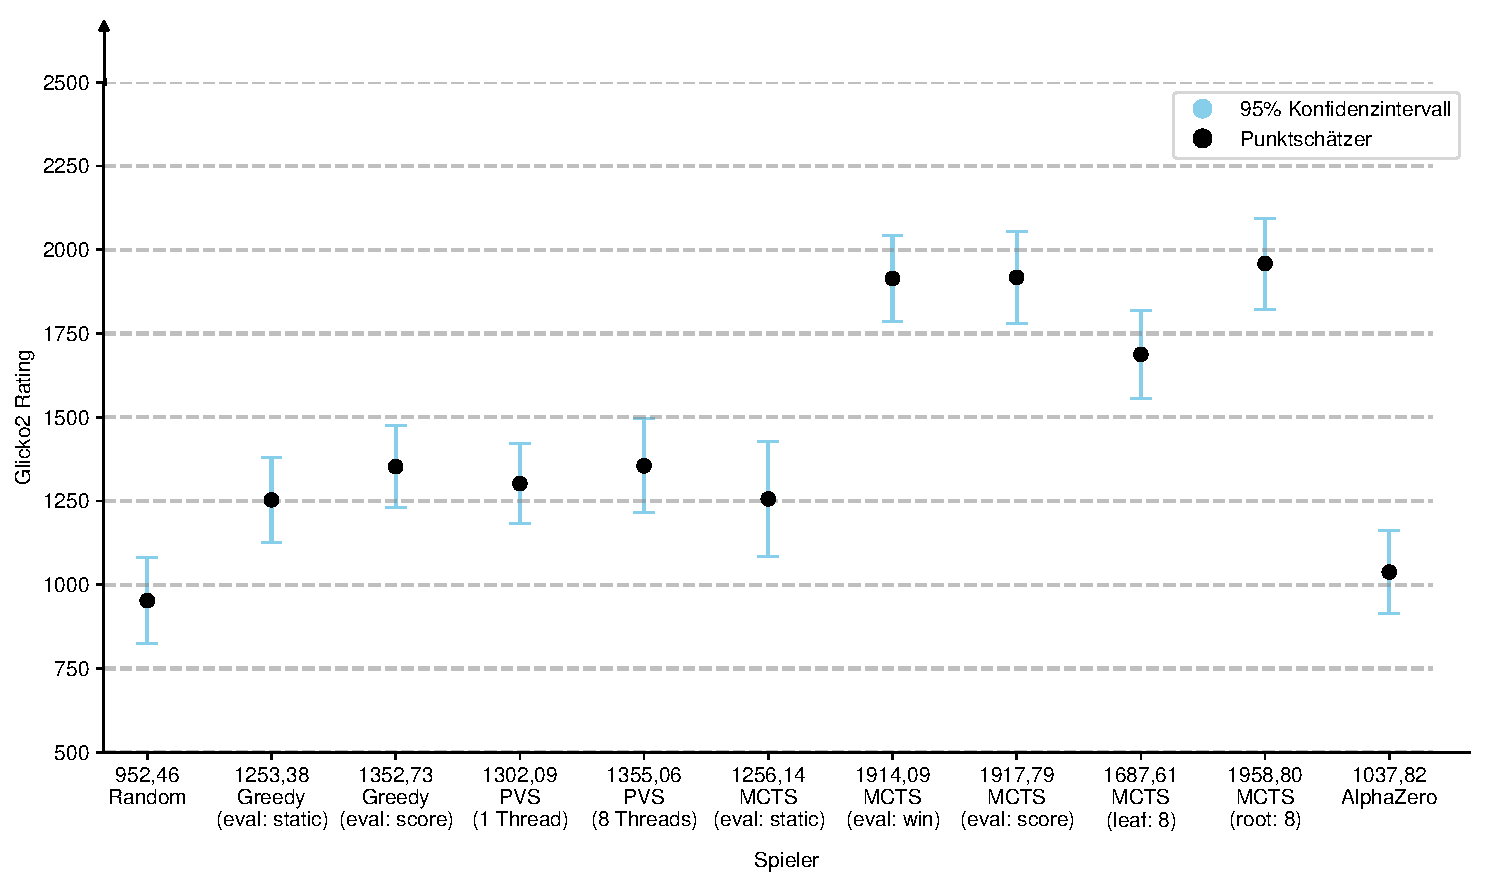
\includegraphics[width=\textwidth]{res/pictures/plots/player-ratings.pdf}
    \caption{Bewertung der Spieler im Glicko-2-Wertungssystem}
    \label{fig:player-ratings}
\end{figure}

In der Rangliste spiegeln sich die Ergebnisse der Vergleichspartien. Auch hier ist der RandomPlayer der schlechteste Spieler. Kurz davor liegt PatchZero. Die Greedy und \ac{PVS} Spieler Varianten teilen sich zusammen in eine ähnliche Bewertungsgruppe ein, wobei der mit Lazy \ac{SMP} parallelisierte \ac{PVS} Spieler die Gruppe anführt. Die \ac{MCTS} Varianten stehen deutlich von den anderen Spielern abgesetzt auf den vorderen Plätzen. Nur der \ac{MCTS} Spieler mit einer statischen Evaluation liegt im Bereich von Greedy- und \ac{PVS}-Spieler. Dies ist nicht verwunderlich, da diese Variante auch eher ähnlich zu diesen Spielern arbeitet als die tatsächlichen \ac{MCTS} Spieler. Die \hyperref[text:leaf-parallelization]{\emph{Leaf Parallelisierung}} bei \ac{MCTS} liegt leicht abgeschlagen von den anderen Varianten, jedoch immer noch weit vor allen anderen Algorithmen, während \hyperref[text:root-parallelization]{\emph{Root Parallelisierung}} einen kleinen Rangvorsprung über die Single-Threaded \ac{MCTS} Varianten aufbauen kann. An dieser Stelle ist es wichtig anzumerken, dass alle in Abbildung \ref{fig:player-ratings} aufgezeigten Glicko-2-Ratings nur relativ zueinander sind und somit nicht mit anderen Glicko-2-Ratings, zum Beispiel von Schach, verglichen werden können.

\pagebreak

\section{Ergebnisse gegen die Autoren}

Abschließend wird noch eine \textbf{subjektive} Einschätzung der Spielstärke der einzelnen Computerengines durch die Autoren dieser Arbeit vorgenommen, um die objektivere Einordnung oben zu ergänzen. Dazu wurden verschiedene Spiele gegen die einzelnen Engines gespielt, jedoch nicht genau protokolliert, wie die genauen Ergebnisse aussehen. Die subjektive Einschätzung begrenzt sich dabei jeweils auf die stärkste Variante der unterschiedlichen Computerspielengines.

Gegen den Random Spieler konnten die Autoren einen Großteil der Spiele gewinnen. Generell hat das $7\times 7$ Sonderplättchen für den Random Spieler keinerlei Relevanz, da er immer nur zufällig Flicken über seinen Ablageplan verteilt. So entsteht auf dem Ablageplan der Engine mit sehr hoher Wahrscheinlichkeit eine Zusammenstellung einzelner Fragmente, die untereinander viele Lücken besitzen und keine große gemeinsame Region. Somit erhält der Random Spieler eigentlich nie das $7\times 7$ Sonderplättchen. Für die Autoren dieser Arbeit ist das Sonderplättchen hingegen so gut wie immer erreichbar. Der Punkteunterschied von 7 Punkten, der dadurch am Ende immer existiert, reicht fast immer aus, um das Spiel zu gewinnen. Generell spielt der Random Spieler aber besser als erwartet. Dadurch, dass es in den meisten Fällen deutlich mehr Aktionen gibt, um einen Flicken zu legen (durch alle möglichen Zeilen- und Spaltenpositionen sowie die Rotation und Spiegelung) anstatt die Laufaktion auszuführen, bevorzugt auch der Random Spieler das Legen von Flicken. Somit wird der Ablageplan im Spielverlauf so gut wie möglich gefüllt. Somit erreicht der Random Spieler auch öfters mal Endergebnisse im einstelligen negativen oder positiven Bereich. Solche Ergebnisse lagen auch bei den ersten Spielen der Autoren gegeneinander oft vor.

Die Autoren konnten auch meistens gegen den Greedy Spieler gewinnen. Generell spielt dieser Spieler merklich besser als Random, was sich dadurch auszeichnet, dass die Flickenpositionen auf dem Ablageplan eher wie bei menschlichen Spielern ohne große Lücken sind. Generell wird aber deutlich, dass Greedy dadurch limitiert ist, dass nur eine Position vorausgesehen werden kann. So werden Züge des Gegners nicht beachtet und es findet auch keine längerfristige Planung statt. So schauen sich menschliche Spieler oftmals direkt eine Kombination an Flicken an. Beispielsweise holt ein Spieler sich vielleicht ein schlechteres Teil, um danach direkt noch einmal an der Reihe zu sein und sich ein nun erreichbares besseres Teil zu kaufen.

Der \ac{PVS} Spieler wirkt leicht besser als der Greedy Spieler, was auch mit der Glicko-2 Einschätzung in Abbildung \ref{fig:player-ratings} übereinstimmt. Die Züge wirken teilweise besser überlegt und es werden auch die zuvor angesprochenen Züge mit einer Kombination an Flicken beachtet. Generell können die Autoren aber immer noch gut gegen den \ac{PVS} Spieler gewinnen. Vor allem der Ablageplan des \ac{PVS} Spielers wirkt gegen Ende des Spiels oft noch zu unüberlegt, mit schwierig zu füllenden Lücken. Wahrscheinlich werden durch den statischen Evaluator die Aktionen bevorzugt, die die restlichen Lücken minimieren. Gleichzeitig ist der \ac{PVS} Spieler dann durch die Ebenen, die vorrausgeschaut werden, begrenzt, sodass die Engine nicht mehr erkennt, dass die restlichen übrigen Flicken nicht mehr dazu geeignet sind, um diese Lücken zu füllen.

Bei dem \ac{MCTS} Spieler hingegen sieht es anders aus. Dieser gewinnt oft gegen die Autoren, ist aber merklich durch seine Bedenkzeit von $10\acs{s}$ beschränkt. Das ist vor allem am Spielanfang bemerkbar. Dort werden oft Flicken fast schon zufällig platziert. Oftmals kann ein Spieler beim ersten Zug alle 1345 möglichen Aktionen ausführen. Der \ac{MCTS} schafft dann $50{.}000-100{.}000$ Iterationen während seiner Bedenkzeit, wobei die wahre Anzahl am Anfang eher bei $50{.}000$ Iterationen liegt. Somit ergibt sich eine durchschnittliche Stichprobengröße von nur 37 möglichen Spielverläufen für jede Aktion. Auch wenn der \ac{MCTS} die Stichproben der Spielverläufe nicht gleichverteilt ausprobiert, sondern häufiger gewinnende Aktionen durch die Tree Policy bevorzugt, wirken die $37$ sehr wenig. Dadurch bildet sich am Anfang ein interessanter häufig zufälliger Ablageplan des \ac{MCTS} Spielers. Im Spielverlauf wird der \ac{MCTS} Spieler dann aber immer besser, da durch den gefüllten Ablageplan weniger Aktionen zur Auswahl stehen und die Simulationsphasen bis zum Spielende kürzer dauern. Somit findet der \ac{MCTS} Spieler auch bei diesem Ablageplan durch die große Anzahl an Iterationen immer genau die Züge, die ihm zum Gewinn führen. Für die Autoren wirkt es so, als sehen sie in der Anfangsphase immer besser dar, trotzdem werden die Spiele dann zum Ende hin immer verloren.

Obwohl der PatchZero Spieler nach der Evaluation leicht besser als Random sein sollte, verhält er sich während des Spielgeschehens für die Autoren genau gleich. Somit gewinnen die Autoren hier auch wieder den Großteil der Spiele. Wahrscheinlich liegt dieses Verhalten daran, dass die Engine nicht genug trainiert worden ist und sich für die Netzwerkevaluation als auf die finale Evaluation eigentlich zufällige Werte ergeben. Dabei ist es nicht erkennbar, ob schon erste kleine Dinge gelernt wurden oder ob sich der PatchZero Spieler tatsächlich zufällig verhält.